\documentclass{standalone}
\usepackage{tikz}
\usetikzlibrary{patterns, positioning}
\usepackage[sfdefault]{ClearSans} %% option 'sfdefault' activates Clear Sans as the default text font
\usepackage[T1]{fontenc}

\begin{document}
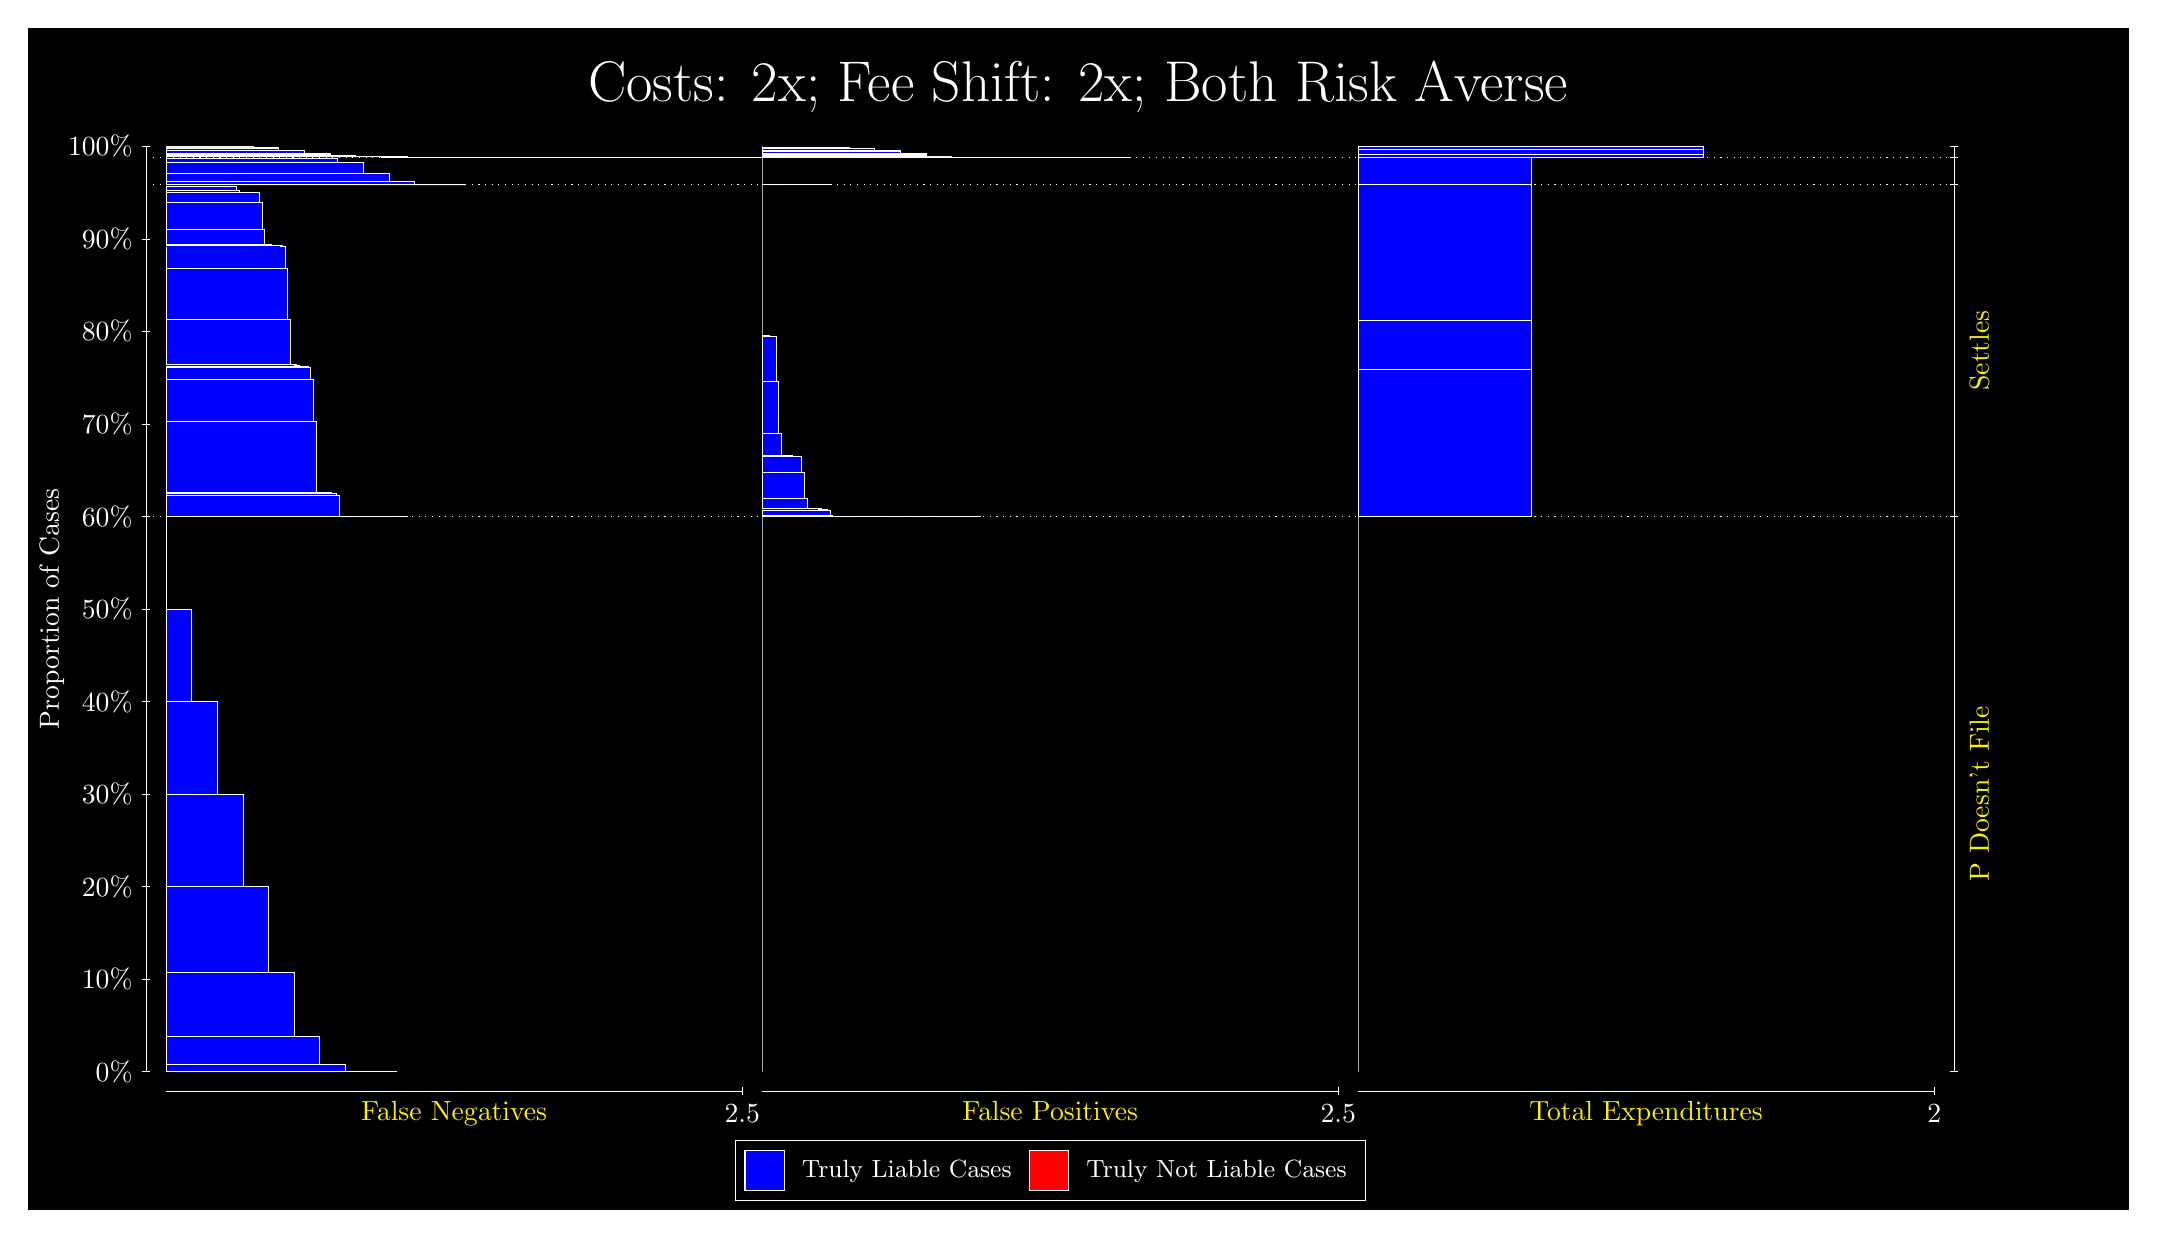
\begin{tikzpicture}
\draw[fill=black] (0,0) rectangle (26.667,15);
\draw[text=white] (0,13.5) rectangle (26.667,15) node[midway] {\huge Costs: 2x; Fee Shift: 2x; Both Risk Averse};
\draw[white, very thin] (1.5,1.75) -- (1.5,13.5);
\node[rotate=90, text=white, anchor=center] at (0.3, 7.625) {Proportion of Cases};
\draw[white, very thin] (1.45,1.75) -- (1.55,1.75);
\node[text=white, anchor=east] at (1.45, 1.75) {0\%};
\draw[white, very thin] (1.45,2.925) -- (1.55,2.925);
\node[text=white, anchor=east] at (1.45, 2.925) {10\%};
\draw[white, very thin] (1.45,4.1) -- (1.55,4.1);
\node[text=white, anchor=east] at (1.45, 4.1) {20\%};
\draw[white, very thin] (1.45,5.275) -- (1.55,5.275);
\node[text=white, anchor=east] at (1.45, 5.275) {30\%};
\draw[white, very thin] (1.45,6.45) -- (1.55,6.45);
\node[text=white, anchor=east] at (1.45, 6.45) {40\%};
\draw[white, very thin] (1.45,7.625) -- (1.55,7.625);
\node[text=white, anchor=east] at (1.45, 7.625) {50\%};
\draw[white, very thin] (1.45,8.8) -- (1.55,8.8);
\node[text=white, anchor=east] at (1.45, 8.8) {60\%};
\draw[white, very thin] (1.45,9.975) -- (1.55,9.975);
\node[text=white, anchor=east] at (1.45, 9.975) {70\%};
\draw[white, very thin] (1.45,11.15) -- (1.55,11.15);
\node[text=white, anchor=east] at (1.45, 11.15) {80\%};
\draw[white, very thin] (1.45,12.325) -- (1.55,12.325);
\node[text=white, anchor=east] at (1.45, 12.325) {90\%};
\draw[white, very thin] (1.45,13.5) -- (1.55,13.5);
\node[text=white, anchor=east] at (1.45, 13.5) {100\%};

\draw[white, very thin] (24.457,1.75) -- (24.457,13.5);
\draw[white, very thin] (24.407,1.75) -- (24.507,1.75);
\node[anchor=west] at (24.407, 1.75) {};
\draw[white, very thin] (24.407,8.8012) -- (24.507,8.8012);
\node[anchor=west] at (24.407, 8.8012) {};
\draw[white, very thin] (24.407,13.013) -- (24.507,13.013);
\node[anchor=west] at (24.407, 13.013) {};
\draw[white, very thin] (24.407,13.359) -- (24.507,13.359);
\node[anchor=west] at (24.407, 13.359) {};
\draw[white, very thin] (24.407,13.361) -- (24.507,13.361);
\node[anchor=west] at (24.407, 13.361) {};
\draw[white, very thin] (24.407,13.5) -- (24.507,13.5);
\node[anchor=west] at (24.407, 13.5) {};

\draw[white, very thin, fill=blue] (1.75,1.75) rectangle (4.6775,1.7504);
\draw[white, very thin, fill=blue] (1.75,1.7504) rectangle (4.3523,1.7582);
\draw[white, very thin, fill=blue] (1.75,1.7582) rectangle (4.027,1.8372);
\draw[white, very thin, fill=blue] (1.75,1.8372) rectangle (3.7017,2.1998);
\draw[white, very thin, fill=blue] (1.75,2.1998) rectangle (3.3764,3.0123);
\draw[white, very thin, fill=blue] (1.75,3.0123) rectangle (3.0511,4.1088);
\draw[white, very thin, fill=blue] (1.75,4.1088) rectangle (2.7258,5.2765);
\draw[white, very thin, fill=blue] (1.75,5.2765) rectangle (2.4006,6.4512);
\draw[white, very thin, fill=blue] (1.75,6.4512) rectangle (2.0753,7.6262);
\draw[white, very thin, fill=red] (1.75,7.6262) rectangle (1.75,7.6262);
\draw[white, very thin, fill=blue] (1.75,7.6262) rectangle (1.75,8.8012);
\draw[white, very thin, fill=blue] (1.75,8.8012) rectangle (4.8239,8.8012);
\draw[white, very thin, fill=blue] (1.75,8.8012) rectangle (4.6775,8.8012);
\draw[white, very thin, fill=blue] (1.75,8.8012) rectangle (4.5312,8.8012);
\draw[white, very thin, fill=blue] (1.75,8.8012) rectangle (4.4986,8.8012);
\draw[white, very thin, fill=blue] (1.75,8.8012) rectangle (4.3848,8.8012);
\draw[white, very thin, fill=blue] (1.75,8.8012) rectangle (4.3523,8.8012);
\draw[white, very thin, fill=blue] (1.75,8.8012) rectangle (4.2384,8.803);
\draw[white, very thin, fill=blue] (1.75,8.803) rectangle (4.2059,8.8031);
\draw[white, very thin, fill=blue] (1.75,8.8031) rectangle (4.1734,8.8031);
\draw[white, very thin, fill=blue] (1.75,8.8031) rectangle (4.092,8.8036);
\draw[white, very thin, fill=blue] (1.75,8.8036) rectangle (4.0595,8.8038);
\draw[white, very thin, fill=blue] (1.75,8.8038) rectangle (4.027,8.8039);
\draw[white, very thin, fill=blue] (1.75,8.8039) rectangle (3.9457,9.0717);
\draw[white, very thin, fill=blue] (1.75,9.0717) rectangle (3.9131,9.098);
\draw[white, very thin, fill=blue] (1.75,9.098) rectangle (3.8806,9.1);
\draw[white, very thin, fill=blue] (1.75,9.1) rectangle (3.8481,9.1006);
\draw[white, very thin, fill=blue] (1.75,9.1006) rectangle (3.7668,9.1042);
\draw[white, very thin, fill=blue] (1.75,9.1042) rectangle (3.7342,9.1068);
\draw[white, very thin, fill=blue] (1.75,9.1068) rectangle (3.7017,9.1078);
\draw[white, very thin, fill=blue] (1.75,9.1078) rectangle (3.6529,10.007);
\draw[white, very thin, fill=blue] (1.75,10.007) rectangle (3.6204,10.541);
\draw[white, very thin, fill=blue] (1.75,10.541) rectangle (3.5878,10.699);
\draw[white, very thin, fill=blue] (1.75,10.699) rectangle (3.5553,10.706);
\draw[white, very thin, fill=blue] (1.75,10.706) rectangle (3.5228,10.708);
\draw[white, very thin, fill=blue] (1.75,10.708) rectangle (3.4415,10.719);
\draw[white, very thin, fill=blue] (1.75,10.719) rectangle (3.4089,10.728);
\draw[white, very thin, fill=blue] (1.75,10.728) rectangle (3.3764,10.729);
\draw[white, very thin, fill=blue] (1.75,10.729) rectangle (3.3276,11.303);
\draw[white, very thin, fill=blue] (1.75,11.303) rectangle (3.2951,11.952);
\draw[white, very thin, fill=blue] (1.75,11.952) rectangle (3.2626,12.233);
\draw[white, very thin, fill=blue] (1.75,12.233) rectangle (3.23,12.238);
\draw[white, very thin, fill=blue] (1.75,12.238) rectangle (3.1975,12.239);
\draw[white, very thin, fill=blue] (1.75,12.239) rectangle (3.1162,12.249);
\draw[white, very thin, fill=blue] (1.75,12.249) rectangle (3.0837,12.255);
\draw[white, very thin, fill=blue] (1.75,12.255) rectangle (3.0511,12.255);
\draw[white, very thin, fill=blue] (1.75,12.255) rectangle (3.0023,12.45);
\draw[white, very thin, fill=blue] (1.75,12.45) rectangle (2.9698,12.785);
\draw[white, very thin, fill=blue] (1.75,12.785) rectangle (2.9373,12.914);
\draw[white, very thin, fill=blue] (1.75,12.914) rectangle (2.9048,12.915);
\draw[white, very thin, fill=blue] (1.75,12.915) rectangle (2.8722,12.915);
\draw[white, very thin, fill=blue] (1.75,12.915) rectangle (2.7909,12.917);
\draw[white, very thin, fill=blue] (1.75,12.917) rectangle (2.7584,12.918);
\draw[white, very thin, fill=blue] (1.75,12.918) rectangle (2.7258,12.918);
\draw[white, very thin, fill=blue] (1.75,12.918) rectangle (2.6771,12.941);
\draw[white, very thin, fill=blue] (1.75,12.941) rectangle (2.6445,12.996);
\draw[white, very thin, fill=blue] (1.75,12.996) rectangle (2.612,13.01);
\draw[white, very thin, fill=blue] (1.75,13.01) rectangle (2.5795,13.01);
\draw[white, very thin, fill=blue] (1.75,13.01) rectangle (2.5469,13.01);
\draw[white, very thin, fill=blue] (1.75,13.01) rectangle (2.4656,13.01);
\draw[white, very thin, fill=blue] (1.75,13.01) rectangle (2.4331,13.01);
\draw[white, very thin, fill=blue] (1.75,13.01) rectangle (2.4006,13.01);
\draw[white, very thin, fill=blue] (1.75,13.01) rectangle (2.3518,13.01);
\draw[white, very thin, fill=blue] (1.75,13.01) rectangle (2.3192,13.013);
\draw[white, very thin, fill=blue] (1.75,13.013) rectangle (2.2867,13.013);
\draw[white, very thin, fill=blue] (1.75,13.013) rectangle (2.2542,13.013);
\draw[white, very thin, fill=blue] (1.75,13.013) rectangle (2.2217,13.013);
\draw[white, very thin, fill=blue] (1.75,13.013) rectangle (2.1403,13.013);
\draw[white, very thin, fill=blue] (1.75,13.013) rectangle (2.1078,13.013);
\draw[white, very thin, fill=blue] (1.75,13.013) rectangle (2.0753,13.013);
\draw[white, very thin, fill=blue] (1.75,13.013) rectangle (2.0265,13.013);
\draw[white, very thin, fill=blue] (1.75,13.013) rectangle (1.994,13.013);
\draw[white, very thin, fill=blue] (1.75,13.013) rectangle (1.9614,13.013);
\draw[white, very thin, fill=blue] (1.75,13.013) rectangle (1.9289,13.013);
\draw[white, very thin, fill=blue] (1.75,13.013) rectangle (1.8964,13.013);
\draw[white, very thin, fill=blue] (1.75,13.013) rectangle (1.8151,13.013);
\draw[white, very thin, fill=blue] (1.75,13.013) rectangle (1.7825,13.013);
\draw[white, very thin, fill=red] (1.75,13.013) rectangle (1.75,13.013);
\draw[white, very thin, fill=blue] (1.75,13.013) rectangle (1.75,13.013);
\draw[white, very thin, fill=blue] (1.75,13.013) rectangle (5.5558,13.014);
\draw[white, very thin, fill=blue] (1.75,13.014) rectangle (5.2305,13.021);
\draw[white, very thin, fill=blue] (1.75,13.021) rectangle (4.9052,13.054);
\draw[white, very thin, fill=blue] (1.75,13.054) rectangle (4.58,13.154);
\draw[white, very thin, fill=blue] (1.75,13.154) rectangle (4.2547,13.295);
\draw[white, very thin, fill=blue] (1.75,13.295) rectangle (3.9294,13.352);
\draw[white, very thin, fill=blue] (1.75,13.352) rectangle (3.6041,13.359);
\draw[white, very thin, fill=blue] (1.75,13.359) rectangle (3.2788,13.359);
\draw[white, very thin, fill=blue] (1.75,13.359) rectangle (2.9535,13.359);
\draw[white, very thin, fill=blue] (1.75,13.359) rectangle (2.6283,13.359);
\draw[white, very thin, fill=red] (1.75,13.359) rectangle (1.75,13.359);
\draw[white, very thin, fill=blue] (1.75,13.359) rectangle (2.6283,13.359);
\draw[white, very thin, fill=blue] (1.75,13.359) rectangle (2.303,13.36);
\draw[white, very thin, fill=blue] (1.75,13.36) rectangle (1.9777,13.361);
\draw[white, very thin, fill=red] (1.75,13.361) rectangle (1.75,13.361);
\draw[white, very thin, fill=blue] (1.75,13.361) rectangle (1.75,13.361);
\draw[white, very thin, fill=blue] (1.75,13.361) rectangle (9.9471,13.361);
\draw[white, very thin, fill=blue] (1.75,13.361) rectangle (9.6218,13.361);
\draw[white, very thin, fill=blue] (1.75,13.361) rectangle (9.2966,13.361);
\draw[white, very thin, fill=blue] (1.75,13.361) rectangle (8.9713,13.361);
\draw[white, very thin, fill=blue] (1.75,13.361) rectangle (8.9713,13.361);
\draw[white, very thin, fill=blue] (1.75,13.361) rectangle (8.646,13.361);
\draw[white, very thin, fill=blue] (1.75,13.361) rectangle (8.3207,13.362);
\draw[white, very thin, fill=blue] (1.75,13.362) rectangle (8.3207,13.362);
\draw[white, very thin, fill=blue] (1.75,13.362) rectangle (7.9954,13.364);
\draw[white, very thin, fill=blue] (1.75,13.364) rectangle (7.9954,13.365);
\draw[white, very thin, fill=blue] (1.75,13.365) rectangle (7.6702,13.367);
\draw[white, very thin, fill=blue] (1.75,13.367) rectangle (7.3449,13.367);
\draw[white, very thin, fill=blue] (1.75,13.367) rectangle (7.3449,13.367);
\draw[white, very thin, fill=blue] (1.75,13.367) rectangle (7.0196,13.367);
\draw[white, very thin, fill=blue] (1.75,13.367) rectangle (6.6943,13.367);
\draw[white, very thin, fill=blue] (1.75,13.367) rectangle (6.369,13.367);
\draw[white, very thin, fill=blue] (1.75,13.367) rectangle (6.369,13.367);
\draw[white, very thin, fill=blue] (1.75,13.367) rectangle (6.0437,13.367);
\draw[white, very thin, fill=blue] (1.75,13.367) rectangle (5.7835,13.367);
\draw[white, very thin, fill=blue] (1.75,13.367) rectangle (5.7185,13.367);
\draw[white, very thin, fill=blue] (1.75,13.367) rectangle (5.4582,13.367);
\draw[white, very thin, fill=blue] (1.75,13.367) rectangle (5.1329,13.367);
\draw[white, very thin, fill=blue] (1.75,13.367) rectangle (4.8077,13.367);
\draw[white, very thin, fill=blue] (1.75,13.367) rectangle (4.8077,13.368);
\draw[white, very thin, fill=blue] (1.75,13.368) rectangle (4.4824,13.37);
\draw[white, very thin, fill=blue] (1.75,13.37) rectangle (4.4824,13.37);
\draw[white, very thin, fill=blue] (1.75,13.37) rectangle (4.1571,13.385);
\draw[white, very thin, fill=blue] (1.75,13.385) rectangle (3.8318,13.4);
\draw[white, very thin, fill=blue] (1.75,13.4) rectangle (3.8318,13.416);
\draw[white, very thin, fill=blue] (1.75,13.416) rectangle (3.5065,13.454);
\draw[white, very thin, fill=blue] (1.75,13.454) rectangle (3.1812,13.469);
\draw[white, very thin, fill=blue] (1.75,13.469) rectangle (3.1812,13.469);
\draw[white, very thin, fill=blue] (1.75,13.469) rectangle (3.1812,13.484);
\draw[white, very thin, fill=blue] (1.75,13.484) rectangle (2.856,13.497);
\draw[white, very thin, fill=blue] (1.75,13.497) rectangle (2.856,13.497);
\draw[white, very thin, fill=blue] (1.75,13.497) rectangle (2.5307,13.498);
\draw[white, very thin, fill=blue] (1.75,13.498) rectangle (2.5307,13.498);
\draw[white, very thin, fill=blue] (1.75,13.498) rectangle (2.5307,13.5);
\draw[white, very thin, fill=blue] (1.75,13.5) rectangle (2.2054,13.5);
\draw[white, very thin, fill=blue] (1.75,13.5) rectangle (2.2054,13.5);
\draw[white, very thin, fill=blue] (1.75,13.5) rectangle (1.8801,13.5);
\draw[white, very thin, fill=blue] (1.75,13.5) rectangle (1.8801,13.5);
\draw[white, very thin, fill=red] (1.75,13.5) rectangle (1.75,13.5);
\draw[white, very thin, fill=blue] (1.75,13.5) rectangle (1.75,13.5);
\draw[white, very thin, fill=red] (9.3189,1.75) rectangle (9.3189,1.75);
\draw[white, very thin, fill=blue] (9.3189,1.75) rectangle (9.3189,8.8012);
\draw[white, very thin, fill=red] (9.3189,8.8012) rectangle (12.1,8.8012);
\draw[white, very thin, fill=blue] (9.3189,8.8012) rectangle (12.1,8.8012);
\draw[white, very thin, fill=red] (9.3189,8.8012) rectangle (11.807,8.8012);
\draw[white, very thin, fill=blue] (9.3189,8.8012) rectangle (11.807,8.8012);
\draw[white, very thin, fill=blue] (9.3189,8.8012) rectangle (11.775,8.8012);
\draw[white, very thin, fill=red] (9.3189,8.8012) rectangle (11.661,8.8012);
\draw[white, very thin, fill=blue] (9.3189,8.8012) rectangle (11.661,8.8012);
\draw[white, very thin, fill=red] (9.3189,8.8012) rectangle (11.515,8.8012);
\draw[white, very thin, fill=blue] (9.3189,8.8012) rectangle (11.515,8.8012);
\draw[white, very thin, fill=blue] (9.3189,8.8012) rectangle (11.482,8.8012);
\draw[white, very thin, fill=blue] (9.3189,8.8012) rectangle (11.449,8.8012);
\draw[white, very thin, fill=red] (9.3189,8.8012) rectangle (11.368,8.8012);
\draw[white, very thin, fill=blue] (9.3189,8.8012) rectangle (11.368,8.8012);
\draw[white, very thin, fill=blue] (9.3189,8.8012) rectangle (11.336,8.8012);
\draw[white, very thin, fill=red] (9.3189,8.8012) rectangle (11.222,8.8012);
\draw[white, very thin, fill=blue] (9.3189,8.8012) rectangle (11.222,8.8012);
\draw[white, very thin, fill=blue] (9.3189,8.8012) rectangle (11.189,8.8012);
\draw[white, very thin, fill=blue] (9.3189,8.8012) rectangle (11.157,8.8012);
\draw[white, very thin, fill=blue] (9.3189,8.8012) rectangle (11.124,8.8012);
\draw[white, very thin, fill=red] (9.3189,8.8012) rectangle (11.075,8.8012);
\draw[white, very thin, fill=blue] (9.3189,8.8012) rectangle (11.075,8.8012);
\draw[white, very thin, fill=blue] (9.3189,8.8012) rectangle (11.043,8.8012);
\draw[white, very thin, fill=blue] (9.3189,8.8012) rectangle (11.01,8.8012);
\draw[white, very thin, fill=red] (9.3189,8.8012) rectangle (10.929,8.8012);
\draw[white, very thin, fill=blue] (9.3189,8.8012) rectangle (10.929,8.8012);
\draw[white, very thin, fill=blue] (9.3189,8.8012) rectangle (10.896,8.8012);
\draw[white, very thin, fill=blue] (9.3189,8.8012) rectangle (10.864,8.8012);
\draw[white, very thin, fill=blue] (9.3189,8.8012) rectangle (10.831,8.8012);
\draw[white, very thin, fill=blue] (9.3189,8.8012) rectangle (10.799,8.8012);
\draw[white, very thin, fill=blue] (9.3189,8.8012) rectangle (10.75,8.8012);
\draw[white, very thin, fill=blue] (9.3189,8.8012) rectangle (10.718,8.8012);
\draw[white, very thin, fill=blue] (9.3189,8.8012) rectangle (10.685,8.8012);
\draw[white, very thin, fill=blue] (9.3189,8.8012) rectangle (10.604,8.8012);
\draw[white, very thin, fill=blue] (9.3189,8.8012) rectangle (10.571,8.8012);
\draw[white, very thin, fill=blue] (9.3189,8.8012) rectangle (10.539,8.8015);
\draw[white, very thin, fill=blue] (9.3189,8.8015) rectangle (10.506,8.8037);
\draw[white, very thin, fill=blue] (9.3189,8.8037) rectangle (10.474,8.8044);
\draw[white, very thin, fill=blue] (9.3189,8.8044) rectangle (10.425,8.8044);
\draw[white, very thin, fill=blue] (9.3189,8.8044) rectangle (10.392,8.8045);
\draw[white, very thin, fill=blue] (9.3189,8.8045) rectangle (10.36,8.8046);
\draw[white, very thin, fill=blue] (9.3189,8.8046) rectangle (10.278,8.8046);
\draw[white, very thin, fill=blue] (9.3189,8.8046) rectangle (10.246,8.8046);
\draw[white, very thin, fill=blue] (9.3189,8.8046) rectangle (10.213,8.8181);
\draw[white, very thin, fill=blue] (9.3189,8.8181) rectangle (10.181,8.8729);
\draw[white, very thin, fill=blue] (9.3189,8.8729) rectangle (10.148,8.8964);
\draw[white, very thin, fill=blue] (9.3189,8.8964) rectangle (10.1,8.8964);
\draw[white, very thin, fill=blue] (9.3189,8.8964) rectangle (10.067,8.8971);
\draw[white, very thin, fill=blue] (9.3189,8.8971) rectangle (10.034,8.8994);
\draw[white, very thin, fill=blue] (9.3189,8.8994) rectangle (9.9532,8.8995);
\draw[white, very thin, fill=blue] (9.3189,8.8995) rectangle (9.9206,8.9002);
\draw[white, very thin, fill=blue] (9.3189,8.9002) rectangle (9.8881,9.0291);
\draw[white, very thin, fill=blue] (9.3189,9.0291) rectangle (9.8556,9.3637);
\draw[white, very thin, fill=blue] (9.3189,9.3637) rectangle (9.8231,9.5591);
\draw[white, very thin, fill=blue] (9.3189,9.5591) rectangle (9.7743,9.5593);
\draw[white, very thin, fill=blue] (9.3189,9.5593) rectangle (9.7417,9.5647);
\draw[white, very thin, fill=blue] (9.3189,9.5647) rectangle (9.7092,9.575);
\draw[white, very thin, fill=blue] (9.3189,9.575) rectangle (9.6279,9.5759);
\draw[white, very thin, fill=blue] (9.3189,9.5759) rectangle (9.5954,9.581);
\draw[white, very thin, fill=blue] (9.3189,9.581) rectangle (9.5628,9.862);
\draw[white, very thin, fill=blue] (9.3189,9.862) rectangle (9.5303,10.511);
\draw[white, very thin, fill=blue] (9.3189,10.511) rectangle (9.4978,11.086);
\draw[white, very thin, fill=blue] (9.3189,11.086) rectangle (9.449,11.087);
\draw[white, very thin, fill=blue] (9.3189,11.087) rectangle (9.4165,11.095);
\draw[white, very thin, fill=blue] (9.3189,11.095) rectangle (9.3839,11.106);
\draw[white, very thin, fill=blue] (9.3189,11.106) rectangle (9.3189,13.013);
\draw[white, very thin, fill=red] (9.3189,13.013) rectangle (10.197,13.013);
\draw[white, very thin, fill=blue] (9.3189,13.013) rectangle (10.197,13.013);
\draw[white, very thin, fill=blue] (9.3189,13.013) rectangle (9.8718,13.013);
\draw[white, very thin, fill=blue] (9.3189,13.013) rectangle (9.5466,13.013);
\draw[white, very thin, fill=blue] (9.3189,13.013) rectangle (9.3189,13.359);
\draw[white, very thin, fill=red] (9.3189,13.359) rectangle (13.125,13.359);
\draw[white, very thin, fill=blue] (9.3189,13.359) rectangle (13.125,13.359);
\draw[white, very thin, fill=blue] (9.3189,13.359) rectangle (12.799,13.359);
\draw[white, very thin, fill=blue] (9.3189,13.359) rectangle (12.474,13.359);
\draw[white, very thin, fill=blue] (9.3189,13.359) rectangle (12.149,13.359);
\draw[white, very thin, fill=blue] (9.3189,13.359) rectangle (11.824,13.359);
\draw[white, very thin, fill=blue] (9.3189,13.359) rectangle (11.498,13.359);
\draw[white, very thin, fill=blue] (9.3189,13.359) rectangle (11.173,13.359);
\draw[white, very thin, fill=blue] (9.3189,13.359) rectangle (10.848,13.36);
\draw[white, very thin, fill=blue] (9.3189,13.36) rectangle (10.522,13.361);
\draw[white, very thin, fill=blue] (9.3189,13.361) rectangle (10.197,13.361);
\draw[white, very thin, fill=red] (9.3189,13.361) rectangle (14.003,13.361);
\draw[white, very thin, fill=blue] (9.3189,13.361) rectangle (14.003,13.361);
\draw[white, very thin, fill=red] (9.3189,13.361) rectangle (13.678,13.361);
\draw[white, very thin, fill=blue] (9.3189,13.361) rectangle (13.678,13.361);
\draw[white, very thin, fill=red] (9.3189,13.361) rectangle (13.352,13.361);
\draw[white, very thin, fill=blue] (9.3189,13.361) rectangle (13.352,13.361);
\draw[white, very thin, fill=blue] (9.3189,13.361) rectangle (13.027,13.361);
\draw[white, very thin, fill=red] (9.3189,13.361) rectangle (13.027,13.361);
\draw[white, very thin, fill=blue] (9.3189,13.361) rectangle (13.027,13.361);
\draw[white, very thin, fill=blue] (9.3189,13.361) rectangle (12.702,13.361);
\draw[white, very thin, fill=red] (9.3189,13.361) rectangle (12.702,13.361);
\draw[white, very thin, fill=blue] (9.3189,13.361) rectangle (12.702,13.361);
\draw[white, very thin, fill=blue] (9.3189,13.361) rectangle (12.377,13.361);
\draw[white, very thin, fill=red] (9.3189,13.361) rectangle (12.377,13.361);
\draw[white, very thin, fill=blue] (9.3189,13.361) rectangle (12.377,13.361);
\draw[white, very thin, fill=blue] (9.3189,13.361) rectangle (12.051,13.363);
\draw[white, very thin, fill=red] (9.3189,13.363) rectangle (12.051,13.363);
\draw[white, very thin, fill=blue] (9.3189,13.363) rectangle (12.051,13.364);
\draw[white, very thin, fill=blue] (9.3189,13.364) rectangle (12.051,13.364);
\draw[white, very thin, fill=blue] (9.3189,13.364) rectangle (12.051,13.364);
\draw[white, very thin, fill=blue] (9.3189,13.364) rectangle (11.726,13.374);
\draw[white, very thin, fill=red] (9.3189,13.374) rectangle (11.726,13.374);
\draw[white, very thin, fill=blue] (9.3189,13.374) rectangle (11.726,13.377);
\draw[white, very thin, fill=blue] (9.3189,13.377) rectangle (11.726,13.377);
\draw[white, very thin, fill=blue] (9.3189,13.377) rectangle (11.401,13.382);
\draw[white, very thin, fill=blue] (9.3189,13.382) rectangle (11.401,13.401);
\draw[white, very thin, fill=blue] (9.3189,13.401) rectangle (11.401,13.407);
\draw[white, very thin, fill=blue] (9.3189,13.407) rectangle (11.075,13.415);
\draw[white, very thin, fill=blue] (9.3189,13.415) rectangle (11.075,13.439);
\draw[white, very thin, fill=blue] (9.3189,13.439) rectangle (11.075,13.445);
\draw[white, very thin, fill=blue] (9.3189,13.445) rectangle (10.75,13.453);
\draw[white, very thin, fill=blue] (9.3189,13.453) rectangle (10.75,13.453);
\draw[white, very thin, fill=blue] (9.3189,13.453) rectangle (10.75,13.472);
\draw[white, very thin, fill=blue] (9.3189,13.472) rectangle (10.75,13.476);
\draw[white, very thin, fill=blue] (9.3189,13.476) rectangle (10.425,13.482);
\draw[white, very thin, fill=blue] (9.3189,13.482) rectangle (10.425,13.491);
\draw[white, very thin, fill=blue] (9.3189,13.491) rectangle (10.1,13.491);
\draw[white, very thin, fill=blue] (9.3189,13.491) rectangle (10.1,13.493);
\draw[white, very thin, fill=blue] (9.3189,13.493) rectangle (10.1,13.493);
\draw[white, very thin, fill=blue] (9.3189,13.493) rectangle (9.7743,13.494);
\draw[white, very thin, fill=blue] (9.3189,13.494) rectangle (9.7743,13.494);
\draw[white, very thin, fill=blue] (9.3189,13.494) rectangle (9.449,13.494);
\draw[white, very thin, fill=blue] (9.3189,13.494) rectangle (9.449,13.494);
\draw[white, very thin, fill=blue] (9.3189,13.494) rectangle (9.449,13.494);
\draw[white, very thin, fill=red] (9.3189,13.494) rectangle (9.3189,13.494);
\draw[white, very thin, fill=blue] (9.3189,13.494) rectangle (9.3189,13.5);
\draw[white, very thin, fill=red] (16.888,1.75) rectangle (16.888,1.75);
\draw[white, very thin, fill=blue] (16.888,1.75) rectangle (16.888,8.8012);
\draw[white, very thin, fill=red] (16.888,8.8012) rectangle (19.083,8.8012);
\draw[white, very thin, fill=blue] (16.888,8.8012) rectangle (19.083,10.674);
\draw[white, very thin, fill=red] (16.888,10.674) rectangle (19.083,10.674);
\draw[white, very thin, fill=blue] (16.888,10.674) rectangle (19.083,11.286);
\draw[white, very thin, fill=red] (16.888,11.286) rectangle (19.083,11.286);
\draw[white, very thin, fill=blue] (16.888,11.286) rectangle (19.083,13.013);
\draw[white, very thin, fill=red] (16.888,13.013) rectangle (19.083,13.013);
\draw[white, very thin, fill=blue] (16.888,13.013) rectangle (19.083,13.359);
\draw[white, very thin, fill=red] (16.888,13.359) rectangle (19.083,13.359);
\draw[white, very thin, fill=blue] (16.888,13.359) rectangle (19.083,13.361);
\draw[white, very thin, fill=red] (16.888,13.361) rectangle (21.279,13.361);
\draw[white, very thin, fill=blue] (16.888,13.361) rectangle (21.279,13.398);
\draw[white, very thin, fill=red] (16.888,13.398) rectangle (21.279,13.398);
\draw[white, very thin, fill=blue] (16.888,13.398) rectangle (21.279,13.464);
\draw[white, very thin, fill=red] (16.888,13.464) rectangle (21.279,13.464);
\draw[white, very thin, fill=blue] (16.888,13.464) rectangle (21.279,13.5);
\draw[white, dotted] (1.5,8.8012) -- (24.457,8.8012);
\draw[white, dotted] (1.5,13.013) -- (24.457,13.013);
\draw[white, dotted] (1.5,13.359) -- (24.457,13.359);
\draw[white, dotted] (1.5,13.361) -- (24.457,13.361);
\draw[white, very thin] (1.75,1.5) -- (9.0689,1.5);
\node[text=yellow, anchor=north] at (5.4094, 1.5) {False Negatives};
\draw[white, very thin] (9.0689,1.45) -- (9.0689,1.55);
\node[text=white, anchor=north] at (9.0689, 1.45) {2.5};

\draw[white, very thin] (9.3189,1.5) -- (16.638,1.5);
\node[text=yellow, anchor=north] at (12.978, 1.5) {False Positives};
\draw[white, very thin] (16.638,1.45) -- (16.638,1.55);
\node[text=white, anchor=north] at (16.638, 1.45) {2.5};

\draw[white, very thin] (16.888,1.5) -- (24.207,1.5);
\node[text=yellow, anchor=north] at (20.547, 1.5) {Total Expenditures};
\draw[white, very thin] (24.207,1.45) -- (24.207,1.55);
\node[text=white, anchor=north] at (24.207, 1.45) {2};

\node[text=yellow, centered, rotate=90] at (24.777, 5.2756) {P Doesn't File};
\node[text=yellow, centered, rotate=90] at (24.777, 10.907) {Settles};




\draw (12.978300999999998,1.5) node[draw=none] (baseCoordinate) {};
\begin{scope}[align=center]
        \matrix[scale=0.5, draw=white, below=0.5cm of baseCoordinate, nodes={draw}, column sep=0.1cm]{
            \node[rectangle, draw, minimum width=0.5cm, minimum height=0.5cm, fill=blue] {}; &
            \node[draw=none, font=\small, text=white] (B) {Truly Liable Cases}; &
            \node[rectangle, draw, minimum width=0.5cm, minimum height=0.5cm, fill=red] {}; &
            \node[draw=none, font=\small, text=white] (B) {Truly Not Liable Cases}; \\
            };
\end{scope}

\end{tikzpicture}
\end{document}